% @File    : c:\Users\Administrator\Desktop\GNN\tutorial\tutorial.tex
 % @Date    : 2020-12-05 22:34:41
 % @Author  : RankFan
 % @Email   : 1917703489@qq.com
 % -----
 % Last Modified: 2020-12-06 20:23:04
 % Modified By: Rank_fan
 % -----
 %%%%%%%%%%%%%%%%%%%%%%%%%%%%%%%%%%%%%%%%%% 

 \documentclass[11pt]{article}
 
 \usepackage{ctex}
%  \usepackage{amsthm}
 \usepackage{amsmath}
 \usepackage{booktabs}
 \usepackage{amsthm}
%  \usepackage{ntheorem}
 \usepackage{xcolor}
 \usepackage{graphicx}
 \usepackage{amssymb}
 \usepackage{authblk}
 \usepackage{tikz}
 
 \tikzset{>=stealth}
 \usetikzlibrary{arrows,shapes,positioning,matrix}

 \usepackage[left=2cm,right=2cm,top=2.5cm,bottom=3cm]{geometry}
 \usepackage[bookmarks, bookmarksnumbered ,colorlinks, linkcolor = blue, citecolor = myred ]{hyperref}
 \definecolor{myred}{rgb}{153, 0, 0}

 \newcommand*{\email}[1]{%
    \normalsize\href{mailto:#1}{#1}\par
    }
    \newcommand{\tikzmark}[3][]
    {\tikz[remember picture, baseline]
      \node [anchor=base,#1](#2) {#3};}





 \numberwithin{equation}{section}
 \numberwithin{figure}{section}

 \graphicspath{{figures/}}

 %%================================== 设置中文字体 ================================%
\xeCJKsetup{AutoFakeBold=true}
\setCJKmainfont{FZShuSong-Z01}[BoldFont={FZHei-B01},ItalicFont={FZKai-Z03}]
%\setCJKmainfont{FZHei-B01}
\setCJKsansfont{FZHei-B01}
\setCJKmonofont{FZShuSong-Z01}
% \setCJKfamilyfont{zhfs}{FZFangSong-Z02}
% \setCJKfamilyfont{zhli}{FZLiShu-S01}
% \setCJKfamilyfont{zxzt}{FZShuSong-Z01}
% \setCJKfamilyfont{FZDH}{FZHei-B01}
%\newcommand*{\fangsong}{\CJKfamily{zhfs}}
%================================== 设置英文字体 ================================%TeX Gyre Pagella
%\setmainfont[Mapping=tex-text]{Times New Roman}%--------------------------------英文衬线字体
\setmainfont{TeX Gyre Pagella}

 \title{Graph Neutral Networks}
 \author{Rank}
 \affil{公众号:经济知识综合 \\ \email{fanxiaolong98@gmail.com}}
 
 \begin{document}
%================================== 自定义样式 
 \newtheoremstyle{mydef}% name
 {\topsep}% measure of space to leave above the theorem. E.g.: 3pt
 {\topsep}% measure of space to leave below the theorem. E.g.: 3pt
 {\upshape}% name of font to use in the body of the theorem
 {0.5pt}% measure of space to indent
 {\bfseries}% name of head font
 {: }% punctuation between head and body
 { }% space after theorem head; " " = normal interword space
 {\thmname{#1}\thmnumber{ #2}\thmnote{ (#3)}}

\theoremstyle{mydef}

\newtheorem{myExample}{Example}[section]
\newtheorem{myRemark}{Remark}[section]
\newtheorem{mydef}{Definiton}[section]

    \maketitle
    \tableofcontents
    \newpage
    \section{Embedding}

CNN 中的卷积就是一种离散卷积,本质上就是利用一个共享参数的过滤器(Kernel)。图数
据和图像数据的差别在于节点邻居个数、次序都是不定的。

生活中很多数据不具备规则的空间结构,称为Non Euclidean data,如,推荐系统、电子交易、分子结构等抽象出来的图谱。流形也是典型的非欧结构。
\begin{itemize}
    \item 1D:社交网络(eg:Facebook,Twitter等)
    \item 2D:生物网络(基因,分子,大脑连接)等
    \item 3D:基础设施网络(eg:能源,交通,互联网,通信等)
\end{itemize}

社交网络非常适合用图数据来表达,社交网络中节点以及节点与节点之间的关系,用户A(有ID信息等)、用户B、帖子都是节点,用户与用户之间的关系是关注,用户与帖子之间的关系可能是发布或者转发。

图的空间结构特征:
\begin{itemize}
    \item  节点特征:每个节点有自己的特征;(体现在点上)
    \item  结构特征:图数据中的每个节点具有结构特征,即节点与节点存在一定的联系。(体现在边上)
\end{itemize}

图卷积的核心思想是利用『边的信息』(Edge)对『节点信息』(Vertex)进行『聚合』(Aggregate)从而生成新的『节点表示』。

图神经网络将深度学习方法延伸到非欧几里得的图数据上,大大提高了图数据应用的精度。

\begin{myExample}
    对于一个简单的电商的图,其包含卖家,商品和用户三个关键节点,其中,商品节点关联商品类别节点,用户节点关联注册 IP 节点和 注册地址节点。当用户在购买商品时,用户节点和商品节点就会关联交易节点,同时,交易节点也会关联用户下单时所对应的 IP 节点以及收获地址节点,对应的图结构如下图所示。
    \begin{figure}[htb!]
        \centering
        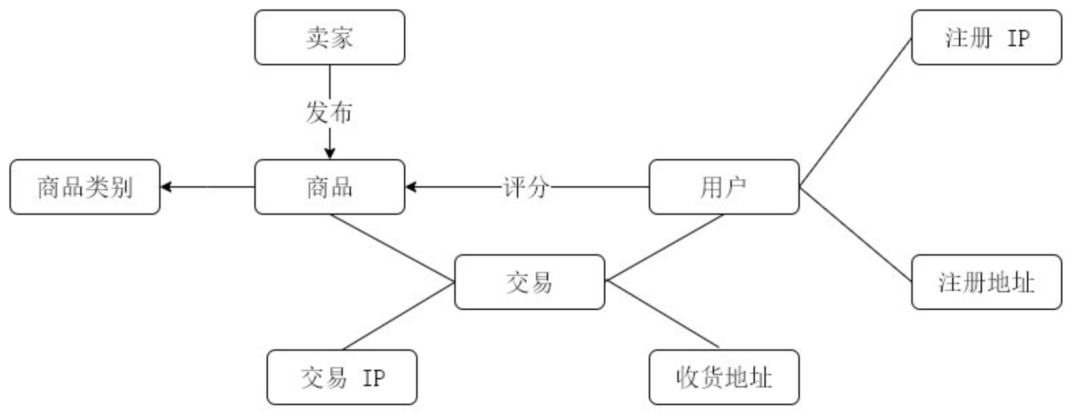
\includegraphics[scale = 0.35]{goods.png}
        \caption{卖家 \& 商品 \& 用户关系图 }
    \end{figure}
    \begin{itemize}
        \item  节点分类—反欺诈:图中每个节点都拥有自己的特征信息,通过该特征信息,我们可以构建一个风控系统,如果交易节点所关联的用户 IP 和收货地址与用户注册 IP 和注册地址不匹配,那么系统将有可能认为该用户存在欺诈风险。
        \item  边结构预测—商品推荐:图中每个节点都具有结构信息。如果用户频繁购买某种类别商品或对某种类别商品评分较高,那么系统就可以认定该用户对该类商品比较感兴趣,
    \end{itemize}
\end{myExample}

    \section{Convolution}

在泛函分析中,卷积是通过两个函数$f(x)$和$g(x)$生成第三个函数的一种算子,它代表的意义是:两个函数中的一个(取$g(x)$,可以任意取)函数,把$g(x)$经过翻转平移,然后与$f(x)$的相乘,得到的一个新的函数,对这个函数积分,也就是对这个新的函数求它所围成的曲边梯形的面积。

设$f(t)$,$g(t)$是两个可积函数,$f(t)$与$g(t)$的卷积记为$f(t) * g(t)$,它是其中一个函数翻转并平移后与另一个函数乘积的积分,是一个自变量是平移量的函数。也就是:

\begin{equation}
    f(t) * g(t)=\int_{-\infty}^{+\infty} f(\tau) g(t-\tau) d \tau=\int_{-\infty}^{+\infty} f(t-\tau) g(\tau) d \tau
\end{equation}

\begin{figure}[htb!]
    \centering
    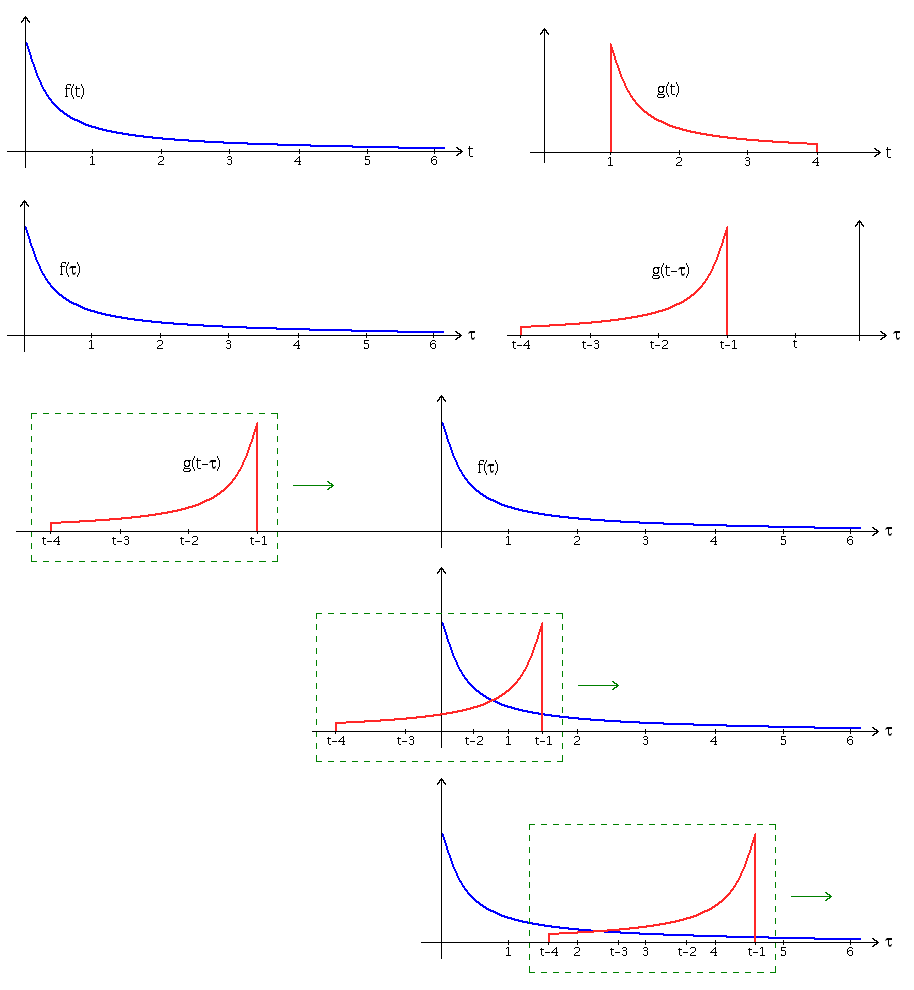
\includegraphics[scale = 0.4]{Convolution3.png}
    \caption{连续卷积图形含义}
\end{figure}

对于定义在整数$\mathbb{Z}$ 上的函数$f,g$卷积定义为:

\begin{equation}
    (f * g)(t)=\sum_{\tau=-\infty}^{\infty} f(\tau) g(t-\tau)
\end{equation}
     %%%%%%%%%%%%%%%%%%%%%%%%%%%%%%%%%%%%%%%%%% 
 % @File    : c:\Users\Administrator\Desktop\GNN\tutorial\sections\Graph-Structure.tex
 % @Date    : 2020-12-08 17:23:06
 % @Author  : RankFan
 % @Email   : 1917703489@qq.com
 % -----
 % Last Modified: 2020-12-14 16:03:43
 % Modified By: Rank_fan
 % -----
 %%%%%%%%%%%%%%%%%%%%%%%%%%%%%%%%%%%%%%%%%% 

\section{Graph Types \& Structures}
     在CNN中,可以将图片转换为RGB的像素矩阵,这种数据可视为时序数据,其他的时序数据还包括语音数据等类型,同时现实中也存在多种信息网络数据,社交网络、金融关系、交通流量网络包括生物学中的蛋白质分子结构,都会涉及大量的高度关联数据。这些数据构成庞大的图,图数据库就是呈现和查询这些关联的做好的方式。

     从数学定义上来说,图是{\bf 节点(vertex,或者 node) }和{\bf 边(Edge)}的集合,在一张图中,一个节点代表一个实体的特征,边,就是关联这些节点的关系 (relation) ,通常这些节点的关系我们会想办法去用数字描述。

     \begin{mydef}[Graph] 
        A graph G is a tuple  $ G = (V, E)  $ of vertices $V$ and edges $E$. For  undirected graphs, edges are subsets of cardinality two of the vertices, so each edge is of the form $(u, v)$ with $u, v \in V$. For directed graphs, the order of the edges in the tuple $(u, v) $is
        relevant to indicate the direction of the edge. If not mentioned otherwise, we will assume
        that a graph is undirected and has no self-loops, i.e. edges for which $u = v$.
     \end{mydef} 

     \begin{mydef}[Degree]
        The degree of a vertex $v$ of an undirected graph $G = (V, E)$ is the number of vertices that are connected to $v$ by means of an edge, i.e. $ deg (v) : 
        \left |  \left \{ u|\left ( u,v \right )  \in E,u \neq v \right \} \right |  $ For directed graphs, a vertex has an {\bf in-degree} and an {\bf out-degree},
        depending on the direction of the edges.
     \end{mydef}

     A graph G = (V, E) may also contain labels or attributes, for example in the form of node labels, edge labels, or edge weights. This is known as an attributed graph.

     \begin{mydef}[Attributed graph]
        {\rm{An attributed graph}} is a graph that has either labels or attributes on the nodes and/or edges. When present, labels are each assumed to be defined
        over a common alphabet, $ \sum_V $ for nodes and $\sum_E$ for edges, with a function, $I_V$ for nodes and $I_E$ for edges, to assign each entity its label. We thus have 
        
        \begin{equation}
            \textstyle 
            \begin{split}
                I_{V} : V \longrightarrow \textstyle  \sum_{V} \\
                I_{E} : E \longrightarrow \textstyle  \sum_{E} 
            \end{split}
        \end{equation}

        and both of these functions need to be total. A graph with additional attributes for verticesand or edges has attribute functions
        \begin{equation}
            \textstyle 
            \begin{split}
                \mathcal{A_{V}}  : V \longrightarrow \textstyle  \mathbb{R}^{d} \\
                \mathcal{A_{V}} : E \longrightarrow \textstyle  \mathbb{  R } ^{d} 
            \end{split}
        \end{equation}

        that are typically assumed to be real-valued, i.e. d = 1. Scalar-valued edge attributes areoften also referred to as weights, with the tacit assumption that the values refer to the strength of a specific connection.

        Since a graph defines a connectivity for each of its vertices, its edges induce sequence. for visiting them. These sequences have specific names, depending on their properties.
     \end{mydef}

     \begin{mydef}[Walks, paths, and cycles]
        A sequence of k nodes  $ v_1 , v_2 , \cdots , v_k $ of the vertices of a graph G is called a walk of length k − 1 if the edge between two consecutive vertices exists.
        Vertices of a walk are allowed to repeat. 
        If, however, node repetition is not allowed, one typically refers to the node sequence as a path, the
        adjective directed often being added in the case of directed graphs. 
        Special consideration is given to cycles, i.e. walks of length k − 1 for which $v_1 = v_k$ .
     \end{mydef}

     \begin{mydef}[Random walks]
        A walk in a graph is referred to as a random walk if the next vertex (or edge) is picked in a probabilistic manner. 
        Having picked a start node at random,a typical choice, for example, would be to pick any outgoing edge of the node with uniform
        probability (in case of unweighted graphs), or with a probability proportional to its weight.
     \end{mydef}

     \begin{mydef}[Connected graph]
        A graph is said to be connected if a walk between all pairs of nodes exists. 
        \begin{myRemark}
            Specifically, in a fully connected graph, each pair of nodes is connected by an edge. If a graph is not connected, the set of its nodes can be partitioned using an equivalence relation u ~ v if and only if a walk between u and v exists. The equivalence classes under this relation are called connected components.

            Likewise, paths can also be used to assess distances in a graph. This viewpoint is oftenhelpful when approximating high-dimensional manifolds through graphs, and it is possible to give bounds on the dissimilarity of graph-based distances and geodesic distances of the manifold .
        \end{myRemark}
     \end{mydef}

     \begin{mydef}[Shortest paths and distances]
        Given two vertices u and v of a graph that are in the same connected component, among all the paths connecting them, there is at least one shortest path that has the minimum number of vertices out of all other paths connecting the two vertices.
     \end{mydef}

     \begin{mydef}[k-hop neighbourhood of a vertex]
        Given a vertex v of a graph G and $ k \in \mathbb{N}_{>0} $ its k-hop neighbourhood  $N^{(k)} (v)$ is defined as all the vertices in G that are reachable
        in at most k steps, which includes v, assuming uniform edge weights.   For example, $N^{(1)} (v)$ is just the set of vertices that are connected to v by an edge and v.
        \begin{myRemark}
            This definition can be connected to the idea of a “ball” in metric spaces by observing that each k-hop neighbourhood of a vertex v induces a subgraph of the original graph G. For increasing values of k, these induced subgraphs are nested—and for k sufficiently large, the original graph G is obtained. This concept will play an important role later on when we define graph kernels that operate at multiple scales,
        \end{myRemark}
     \end{mydef}

     \begin{mydef}[Adjacency matrix A]
        A graph is often represented through its adjacencymatrix A. A graph with n vertices will thus be represented by an n × n binary matrix whose entry Aij = 1 if the ith and jth vertex of the graph are connected by an edge. 
        \begin{myRemark}
            The adjacency matrix is symmetrical for undirected graphs, whereas for directed graphs $A_{ij}$ and $A_{ji}$ can be different depending on the edge structure. Furthermore, if edge weights are available,
            i.e. $\mathcal{A_{E} (\cdot)} $ exists and d = 1, it is also possible to derive a weighted variant of the adjacency
            matrix by setting Aij to the corresponding edge weight.
        \end{myRemark}
     \end{mydef}
     
     \begin{mydef}[Graph Laplacian]
        Let A be the adjacency matrix of a graph G = (V, E).If weights are available, each entry Aij thus consists of the weight of the corresponding edge. Furthermore, let D be the degree matrix of G. This diagonal matrix contains the degree of each vertex $v \in  V $in the unweighted case.  For weighted graphs, each entry consists of the sum of all edge weights of all edges that are incident on the corresponding vertex.Laplacian ,matrix will be a symmetric positive semi-definite matrix for undirected graphs. 
        
        \begin{equation}
            L := D − A
        \end{equation}
     \end{mydef}
\begin{figure}[ht!]
    \centering
    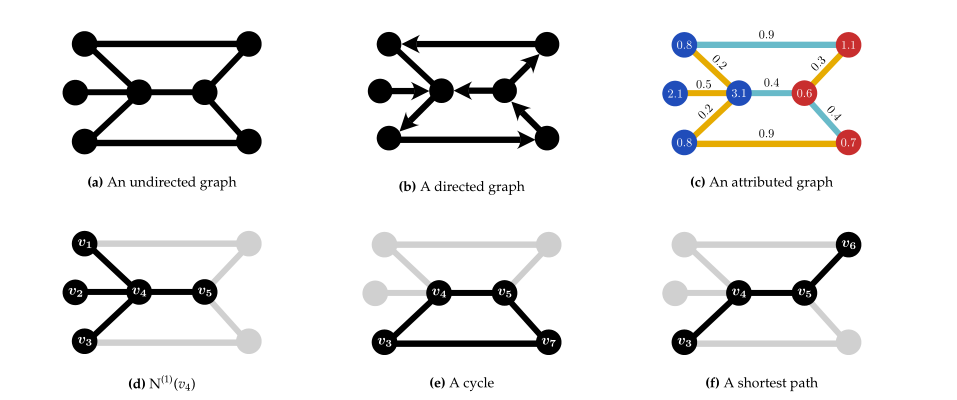
\includegraphics[scale = 0.5]{def_graph.png}
\end{figure}
\begin{figure}[htb!]
    \centering
    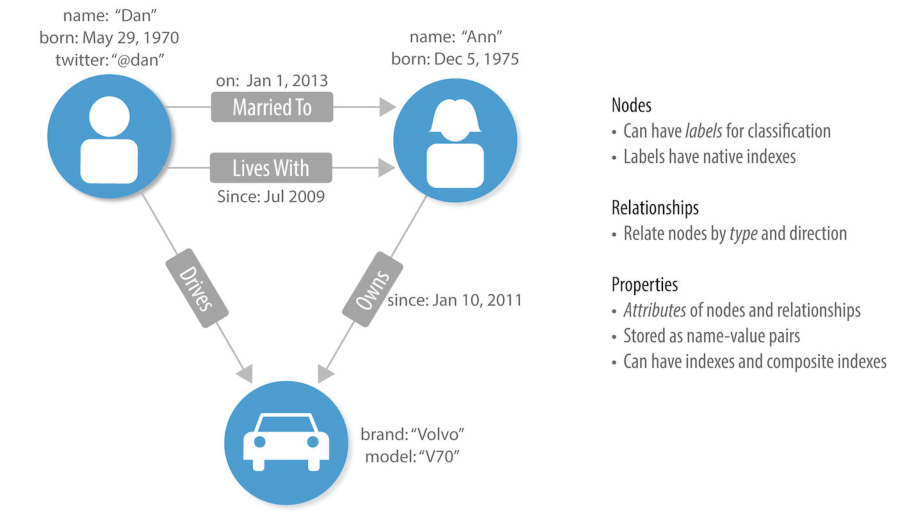
\includegraphics[scale = 0.5]{label_property.png}
    \caption{属性图}
\end{figure}
     %%%%%%%%%%%%%%%%%%%%%%%%%%%%%%%%%%%%%%%%%% 
 % @File    : c:\Users\Administrator\Desktop\GNN\tutorial\sections\GCN-math.tex
 % @Date    : 2020-12-08 17:19:56
 % @Author  : RankFan
 % @Email   : 1917703489@qq.com
 % -----
 % Last Modified: 2020-12-09 15:11:38
 % Modified By: Rank_fan
 % -----
 %%%%%%%%%%%%%%%%%%%%%%%%%%%%%%%%%%%%%%%%%% 

\section{GNN-Math}
     \subsection{Laplace Operator}
     如果 $ f $ 是欧式空间中的二阶可微实函数,那么 $ \Delta \cdot $ (divergence)为拉普拉斯算子, 物理上,散度的意义是场的有源性。 $ \Delta f $ 就是在欧式空间中求其二阶微分({\textbf{散度}})。
     $ div(F)>0 $ 表示该点有散发通量的正源(发散源);$ div(F)= 0 $ 表示该点无源;$ div(F)< 0 $ 表示该点有吸收能量的负源(洞或汇)。
     
     $ \nabla ^{2}f $ 又可以写成  $ \nabla  \cdot \nabla  f $。梯度 “$ \nabla $ ”的本意是一个向量,表示某一个函数在该点处的方向导数沿着该方向取得最大值,即函数的在该方向沿着此方向的梯度方向上升或下降最快



     图的拉普拉斯矩阵,如果把它看作一个线性变换,它起的作用是和数学分析中的拉普拉斯算子是一样的,即拉普拉斯矩阵就是图上的拉普拉斯算子,或者说是离散的拉普拉斯算子。

     如果$ f $ 是图上定义的一组高维向量(特征),那么$ L f $就是在图空间求其二阶微分(散度),$ L $ 是图的拉普拉斯矩阵。

     \begin{myExample}
        $ u = f(x,y) $ 在空间区域 $ G $ 是一阶连续可导($ C ^{1}$) ,点 $ P(x,y) \in G $ 处的梯度向量为:
        \[ \left \{ \frac{\partial f}{\partial x} , \frac{\partial f}{\partial y} 
        \right \}  = \frac{\partial f}{\partial x} \overrightarrow{i} + \frac{\partial f}{\partial y} \overrightarrow{j} \]
        记为$grad \, f(x,y)$ 或 $ \nabla f(x,y)$ 。其中:$ \nabla = \frac{\partial }{\partial x} \overrightarrow{i} + \frac{\partial }{\partial y} \overrightarrow{j}$
        称为(二维)向量的微分算子或 Nabla 算子。
     \end{myExample}

     拉普拉斯算子(Laplace Operator)是 $ n $ 维欧几里得空间中的一个二阶微分算子,定义梯度($ \nabla $ )的散度为 $ \Delta \cdot $ 

     \begin{equation}
        \nabla ^{2}f = \nabla  \cdot \nabla  f  = div(grad \, f )
     \end{equation}

     \begin{myExample}[离散形式的拉普拉斯算子]
        下面以二维为例,每个维度的变化最小单位为1,
        \begin{align*}
            \frac{\partial f}{\partial x} & = f^{\prime} (x) = f(x+1) - f(x) \\
            \frac{\partial^{2} f}{\partial x^{2}} &  =   f^{\prime \prime } (x)   \approx f^{\prime }(x) - f^{\prime }(x-1) 
             = f(x+1) + f(x-1) -2f(x) \\
            \Longrightarrow \Delta f & =   \frac{\partial^{2} f}{\partial x^{2}} +\frac{\partial^{2} f}{\partial y^{2}} \\ 
            & = f(x+1,y) + f(x-1,y) + f(x,y+1) + f(x,y-1) -4f(x,y)  
        \end{align*}
     \end{myExample}
     
     \begin{myRemark}
        如果$ \Delta f = 0 $,可以近似认为中心点 $ f(x,y) $ 的势和其周围点的势是相等的, $ f(x,y) $ 局部范围内不存在势差,所以该点无源。
        如果$ \Delta f > 0 $,可以近似认为中心点 $ f(x,y) $ 的势低于周围点,可以想象成中心点如恒星(太阳)一样发出能量,补给周围的点,所以该点是正源。
        如果$ \Delta f < 0 $,可以近似认为中心点 $ f(x,y) $ 的势高于周围点,可以想象成中心点如吸引子一样在吸收能量,所以该点是负源。
     \end{myRemark}

     另一个角度,拉普拉斯算子计算了周围点与中心点的梯度差。当 $ f(x,y) $  受到扰动之后,其可能变为相邻的$ f(x+1,y) , f(x-1,y) , f(x,y+1) , f(x,y-1)  $之一,拉普拉斯算子得到的是对该点进行微小扰动后可能获得的总\href{https://www.zhihu.com/question/22104055/answer/1236811448}{增益}(或者说是总变化)。

     将这个结论推广到图,假设具有$ N $个节点的图$ G $,此时以上定义的函数f将是$ N $维向量:$ f = (f_1,f_2,f_3,...,f_N) $。其中$ f_i $ 为函数f在图中节点$ i $处函数的值,类比于$ f(x,y) $在节点
     (x,y)处的值。对$ i $ 节点进行扰动,它可能变为任意一个与它相邻的节点 $ j \in N_i $, $ N_i $ 表示节点i的一阶领域点。
     \begin{figure}[htb!]
        \centering
        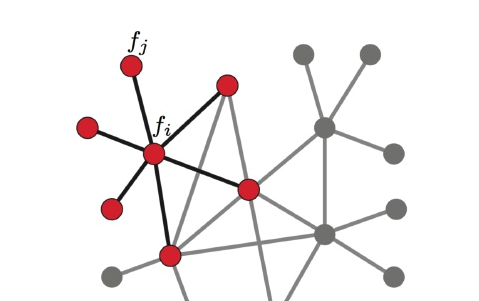
\includegraphics[scale = 0.7 ] {node_graph.png}
        \caption{图结构}
     \end{figure}

     我们上面已经知道拉普拉斯算子可以计算一个点到它所有自由度上微小扰动的增益,则通过图来表示就是任意一个节点 $ j $ 变化到节点$ i $ ,假设图中边的权值相等(简单说就是1 , $ w_{ij} = 1 $)则

     \begin{align*}
         \Delta f_{i} = \sum_{j \in N_{i}} (f_i - f_j) = \sum_{j \in N_{i}} \left [ w_{ij} (f_i - f_j) \right ] 
     \end{align*}

     由于当  $ j \notin  N_{i} \Longrightarrow w_{ij} = 0 $,此时$ i,j $不相邻。
     \begin{align*}
         \sum_{j \in N }  \left [ w_{ij} (f_i - f_j) \right ] &  = \sum_{j \in N } w_{ij}f_i - \sum_{j \in N } w_{ij} f_j \quad d_i \triangleq  \sum_{j \in N } w_{ij}   \\
           & = d_{i} f_{i} -w_{i:}f
    \end{align*}

    $ w_{i:} = (w_{i,1},w_{i,2},\dots,w_{i,N} )$  是$ N $维行向量,$ f = (f_{1},f_{2},\dots,f_{N} )$ 。$ w_{i:}f $ 表示两个向量之间的内积。$ D_{n \times n} $度矩阵,$ W_{n \times n} $ 为邻接矩阵。    $L = D-W $

    \begin{myRemark}
        拉普拉斯矩阵中的第 $ i $ 行实际上反应了第 $ i $ 个节点在对其他所有节点产生扰动时所产生的增益累积。直观上来讲,图拉普拉斯反映了当我们在节点$ i $ 上施加一个势,
        这个势以哪个方向能够多顺畅的流向其他节点(梯度的感觉)。谱聚类中的拉普拉斯矩阵可以理解为是对图的一种矩阵表示形式。
    \end{myRemark}

    \begin{align*}
        \Delta f & =    \left(\begin{array}{c}
            \Delta f_{1} \\
            \vdots \\
            \Delta f_{N}
            \end{array}\right)=\left(\begin{array}{c}
            d_{1} f_{1}-w_{1:} f \\
            \vdots \\
            d_{N} f_{N}-w_{N:} f
            \end{array}\right)  \\
            & =  \left(\begin{array}{ccc}
                d_{1} & \cdots & 0 \\
                \vdots & \ddots & \vdots \\
                0 & \cdots & d_{N}
                \end{array}\right) f-\left(\begin{array}{c}
                w_{1:} \\
                \vdots \\
                w_{N:}
                \end{array}\right) f \\
            & =\operatorname{diag}\left(d_{i}\right) f-W f \\
            & ={\color{myred} (D-W)}f \\
            &={\color{myred} L } f
    \end{align*}


  \subsection{GCN-Spectral Based}       

 
    特征函数与傅里叶算子:
    \begin{align}
        F(w) = \mathcal{F}\left [ f(t) \right ] = \int_{ t } f(t)e^{-iwt}\mathrm{ dt } \\
        e^{-iwt} = cos(wt) - isin(wt) 
    \end{align}
 
    开始我的表演:
    首先 $ \hat{x} = A \boldsymbol x $表示的含义是对x所在的空间进行了转换,如果A的列向量是$ n $个基向量,表示x转换到A的 $ n $个基向量所表征的空间内, $ A \boldsymbol x  = \lambda \boldsymbol x $ ,$ \lambda $是一个scale,这里表示的空间转换仅仅是在
     $ \boldsymbol x $ 进行一个放缩,也就是这个向量($ \boldsymbol x $)是$ A $一个特征向量。
    如果特征向量是基向量,这就意味着进行空间转换也就是对坐标轴进行放缩。

    \begin{align}
        \Delta e^{-iwt} = \frac{\partial^2 e^{-iwt}}{\partial t^2} = \frac{\partial -iwe^{-iwt}}{\partial t} = i^{2} w^{2}e^{-iwt} = -w^{2}e^{-iwt} 
    \end{align}
    
    \[
        \Delta  \tikzmark{identity}{\texttt{ $ e^{-iwt} $ }} = -\tikzmark[red]{G}{ \texttt{$ w^{2} $} }
    \tikzmark[blue]{L}{\texttt{$ e^{-iwt} $}}
    \]
        %  \Delta   \tikzmark{identity}{\texttt{I}}= ( -\tikzmark[red]{G}{ \texttt{G} }
        % \tikzmark[blue]{L}{ \texttt{L} )
  
        % (\tikzmark{identity}{$ \Delta $} \tikzmark[red]{G}{\texttt{G})  = ( -\tikzmark[red]{G}{\texttt{$ w^{2}$}}
        % \tikzmark[blue]{L}{\texttt{$ e^{-iwt} $}} )
    \begin{tikzpicture}[overlay, remember picture,node distance =1.5cm]
        \node (identitydescr) [below left = of identity ]{Eigenvalue};
        \draw[,->,thick] (identitydescr) to [in=-90,out=90] (identity);
        \node[red] (Gdescr) [below right = of G]{Frequency};
        \draw[red,->,thick] (Gdescr) to [in=-90,out=90] (G);
    \end{tikzpicture}

    \begin{align}
        \hat{f} & = u^{T}x \Longrightarrow \hat{y} = {\color{myred} g_{\theta} \star x} = g_{\theta} (\Lambda) \hat{x} =  g_{\theta} (\Lambda) u^{T}x   \Longrightarrow \\
        y  & = \left( u^{T}\right) ^{-1} \hat{y} =  u g_{\theta} (\Lambda)  \hat{x} = g_{\theta} ({\color{myred}u \Lambda u^{T}}) x = g_{\theta} ({\color{myred}L}) x \\
        L_{reg} & =  \sum_{i} \sum_{j} W_{ij}  \left \| f(X_{i}) -f(X_{j}) \right \|  =f ^{T} (X) L f(X) \\
        L & = I_{n} - D^{-\frac{1}{2}}W D^{-\frac{1}{2}} = u \Lambda u^{T}
    \end{align}

    \begin{myRemark}
        $ L _{n \times n}$ 在无向图中是一个实对称阵,实对称阵可对正交对角化,n个不同的特征向量可以表示n个基向量(Independent)。$ u ^ { T } _{ n \times n }f _{n \times 1 }$表示将f所在的空域转换为时域,$g_{\theta} $ 表示一个关于$ \theta $的 $ n \times n $的对角矩阵,其中的参数也就是机器学习要学习的参数。$ \Lambda _{ n \times n }$ 为 L的正交对角化矩阵,$ u u ^ { T }  = I $。

        \[
            \hat{x} =  \begin{pmatrix}
                \hat{f}\left ( {\lambda 1} \right )  \\
                \hat{f}\left ( {\lambda 2} \right )  \\
                \vdots\\
                \hat{f}\left ( {\lambda n} \right )  \\
                
                \end{pmatrix} 
            = \begin{pmatrix}
                u_{1} \left ( 1 \right ) &  u_{1} \left ( 1 \right ) & \cdots&  u_{1} \left ( n \right )& \\
                u_{2} \left ( 1 \right ) &  u_{2} \left ( 2 \right ) & \cdots&  u_{2} \left ( n \right )&\\
               \vdots & \vdots & \vdots &  \vdots& \\
                 u_{n} \left ( 1 \right ) &  u_{n} \left ( 2 \right ) & \cdots&  u_{n} \left ( n \right )&
              \end{pmatrix} 
              \begin{pmatrix}
                f\left ( { 1 } \right )  \\
                f\left ( { 2 } \right ) \\
                \vdots\\
                f\left ( { n } \right )  \\
             \end{pmatrix}\]
        \begin{align*} 
            \hat{f} \left ( {\lambda 1} \right )   & =  u_{1} \left ( 1 \right ) f(1) + u_{1} \left ( 2 \right ) f(2) + \cdots + u_{1} \left ( n \right ) f(n) = \sum_{i = 1} ^{n}  u_{1} \left ( i \right ) x(i) \Longrightarrow \\
            \hat{f\left ( {\lambda_{\ell }} \right )}  & = \sum_{i = 1} ^{n}  u_{\ell } \left ( i \right ) f(i)   = \int u_{\ell } \left ( i \right ) f(i) \mathrm{d i}  \quad \ell  = 1 , 2 ,\dots , n  
        \end{align*}
    \end{myRemark}
    \begin{myExample}[傅里叶逆变换]
    \begin{align*}
        f(t) & = \mathcal{F}^{-1} \left( F(w) \right) = \frac{1}{2\pi} \int F(w) e^{iwt} \mathrm{dw}  \\
        f * h  & = \mathcal{F}^{-1} \left( \hat{f(w)} * \hat{h(w)}  \right) = \frac{1}{2\pi} \int \left( \hat{f(w)} * \hat{h(w)}  \right)  \mathrm{dw} \\
        ( f * h ) _{G}  & = u \, diag\left [  \hat{h(w)} \right ] u^{T} f  =u \, diag\left [   u^{T} h  \right ] u^{T} f  = u \left[  (u^{T} h) \odot (u^{T} f)  \right]
    \end{align*} 
    
        \begin{myRemark}
            $ \odot $ 表示Hadamard product(哈达马积),对于两个维度相同的向量、矩阵、张量进行对应位置的逐元素乘积运算。$ h $ 为卷积核 ,$\hat{h}$ 为 $h$ 的傅里叶变化,这里的 $diag\left [  \hat{h(w)} \right ] $ 是上文中所说的 $g_{\theta} (\Lambda)$ 的另一种形式, $\lambda$ 在频域中和频率表示一个含义。
        \end{myRemark}
        \[
            diag(\hat{h}) = \begin{pmatrix}
                \hat{h(\lambda _{1})} &  0&  0& 0\\
                0&  \hat{h(\lambda _{2})}&  0&0 \\
                \vdots& \vdots & \ddots & \vdots\\
                0& 0 &  0&\hat{h(\lambda _{n})}
              \end{pmatrix}  \]
    \end{myExample}

    \section{GCN}
     %%%%%%%%%%%%%%%%%%%%%%%%%%%%%%%%%%%%%%%%%% 
 % @File    : c:\Users\Administrator\Desktop\GNN\tutorial\sections\GAT.tex
 % @Date    : 2020-12-08 17:20:46
 % @Author  : RankFan
 % @Email   : 1917703489@qq.com
 % -----
 % Last Modified: 2020-12-08 17:20:48
 % Modified By: Rank_fan
 % -----
 %%%%%%%%%%%%%%%%%%%%%%%%%%%%%%%%%%%%%%%%%% 

\section{GAT}
     %%%%%%%%%%%%%%%%%%%%%%%%%%%%%%%%%%%%%%%%%% 
 % @File    : c:\Users\Administrator\Desktop\GNN\tutorial\sections\GraphSAGE.tex
 % @Date    : 2020-12-08 17:21:28
 % @Author  : RankFan
 % @Email   : 1917703489@qq.com
 % -----
 % Last Modified: 2020-12-08 17:21:28
 % Modified By: Rank_fan
 % -----
 %%%%%%%%%%%%%%%%%%%%%%%%%%%%%%%%%%%%%%%%%% 

\section{GraphSAGE}
    \end{document} 